\chapter{Sviluppo dei contenuti}

\section{Attività 1: Introduzione alla ricorsione}

\clm{}{}{Bisogna inzialmente introdurre in linea generale il contenuto
dell'attività agli studenti, facendo attenzione a non perdersi nei dettagli
che verranno approfonditi durante le fasi successive. Questo 
aiuta ad accendere la curiosità degli studenti e a farli partecipare
attivamente all'attività.
}

\nt{In questo documento ho inserito note specifiche per gli insegnanti
(come quella sopra). Tuttavia sono solo brevi suggerimenti, in quanto
la guida per gli insegnanti vera e propria è contenuta nella sezione
seguente. }

\paragraph{Materiale utilizzato in quest'attività:}

\begin{itemize}
    \item [$\Rightarrow$] Lavagna multimediale;
    \item [$\Rightarrow$] Computers.
\end{itemize}

\clm{}{}{In questa fase i computers sono opzionali. Il docente può, a discrezione personale,
decidere di condividere sui computers degli studenti il codice di esempio (per una maggiore interazione)
oppure mostrarlo sulla lavagna multimediale.}

\paragraph{Fase 1:}

\begin{itemize}
    \item [$\Rightarrow$] \textbf{\textcolor{cyan}{Consegna:}} come prima cosa, per introdurre
    quest'attività si consiglia di ripassare brevemente i tipi di dati (Int, float, etc.). 
    Successivamente il docente introduce la ricorsione spiegando i concetti di passo base e passo
    ricorsivo. Per supportare quest'attività si può fare riferimento al primo esercizio di programmazione proposto
    (Fibonacci ricorsivo). Al termine di questa fase si dovranno anche introdurre gli elementi sintattici basilari di Haskell.
    \item [$\Rightarrow$] \textbf{\textcolor{magenta}{Svolgimento:}} inizialmente si presenterà la
    ricorsione in maniera discorsiva anche facendo esempi legati alla quotidianetà 
    (per esempio un \texttt{\href{https://www.researchgate.net/publication/309578166_Percorso_didattico_sulla_ricorsione_dalla_natura_al_coding}{treno}}:
    se ha 1 solo vagone, passo base, allora è semplicemente un vagone. Se ha n > 1 vagoni allora
    è un treno composto da una "testa" e da n - 1 vagoni). Eventualmente si possono anche mostrare,
    su una lavagna multimediale, immagini che presentano la ricorsione (per esempio alcuni dei quadri di Escher
    come "Mani che disegnano" o "Cascata"). Dopo di ché gli studenti verranno incoraggiati a partecipare portando
    ulteriori esempi di ricorsività sulla base delle loro esperienze personali.
     Infine si mostra l'esempio riguardante Fibonacci, scritto in Haskell
    e si approfittà per dare un'idea concreta di utilizzo di ricorsione.
    \item [$\Rightarrow$] \textbf{\textcolor{teal}{Discussione:}} il docente dovrà gestire una discussione
    sulla base degli esempi portati dagli studenti e correggere eventuali errori concettuali
    tramite il dialogo. 
    \item [$\Rightarrow$] \textbf{\textcolor{orange}{Conclusione:}} Per concludere quest'attività il docente introdurrà
    la sintassi base di Haskell (insieme all'utilizzo di GHCI) e si assicurerà che essa venga compresa dagli studenti. 
\end{itemize}

\clm{}{}{Può essere utile, prima di proseguire con l'attività unplugged, porre alcune 
domande agli studenti per assicurarsi che abbiano compreso le basi su cui si sviluppa la ricorsione.
Si può prendere spunto dalla sezione riguardante gli "Indicatori" presente nel capitolo successivo.}

\nt{Comandi utili di GHCI:
\begin{itemize}
    \item \texttt{:load} o \texttt{:l}, serve per compilare un file hs (Haskell);
    \item \texttt{:type} o \texttt{:t}, mostra il tipo di una funzione;
    \item \texttt{:reload} o \texttt{:r}, ricompila tutti i file precedentemente compilati;
    \item \texttt{:!clear}, pulisce lo schermo del terminale di GHCI (solo linux).
\end{itemize}
}

\section{Attività unplugged}\label{unplugged}

\subsection{Attività 2: Le matrioske}

\subsection{Attività 3: Da Unplugged a Programmazione}

\pagebreak

\section{Esercizi di programmazione}\label{prog}

\subsection{Esempio}

\paragraph{Fibonacci ricorsivo:} viene usato nella prima parte dell'attività come esempio
di utilizzo della ricorsione.

\begin{figure}[!h]
    \centering
    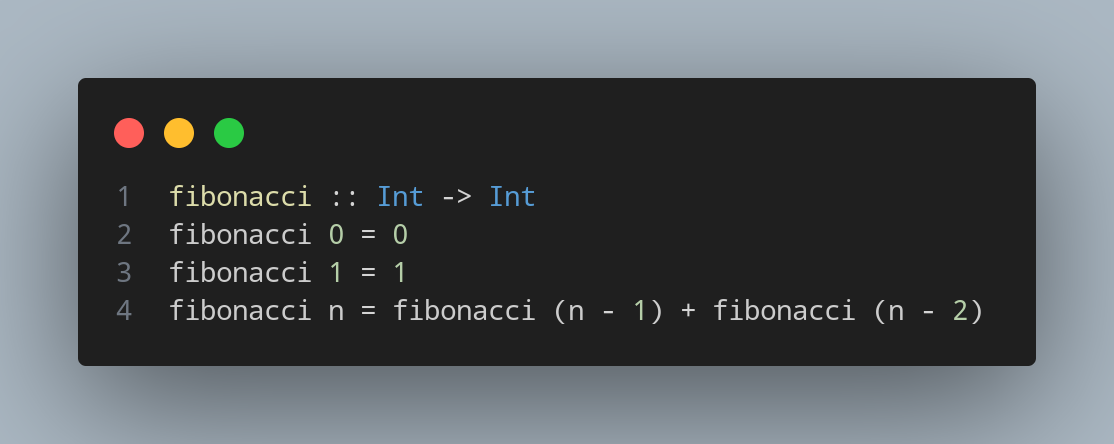
\includegraphics[width=0.5\textwidth]{images/Fibonacci.png}
\end{figure}

\subsection{Esercizi per prendere confidenza}

\paragraph{Somma:} Scrivere una funzione in Haskell (con tipo \texttt{Int -> Int}), 
che prenda in input un intero n e calcoli la somma dei primi n numeri naturali.

\begin{figure}[!h]
    \centering
    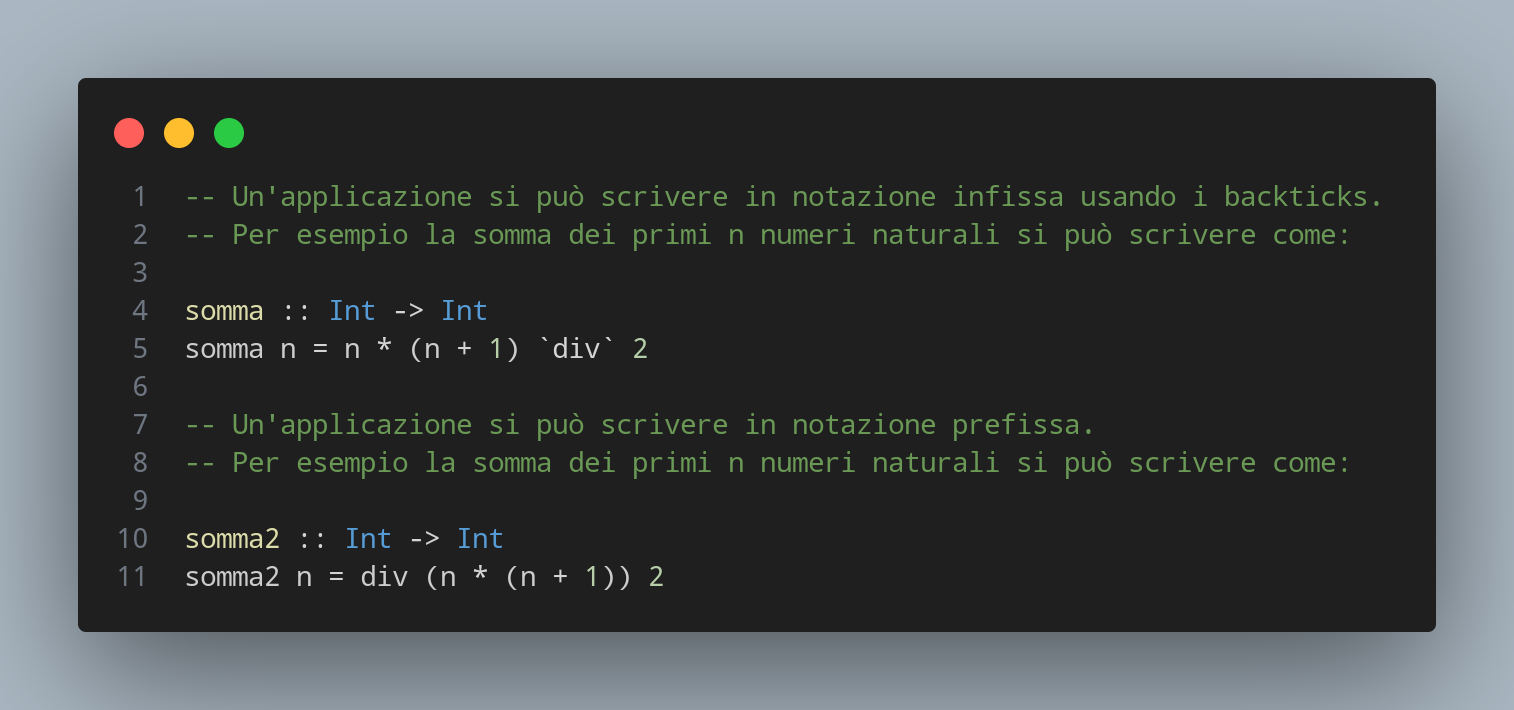
\includegraphics[width=0.8\textwidth]{images/Somma.png}
\end{figure}

\subsection{Esercizi sulle guardie}

\paragraph{Massimo:} Scrivere una funzione in Haskell (con tipo \texttt{Int -> Int -> Int}), usando 
le guardie, che
prenda in input due interi e restituisca il maggiore.

\begin{figure}[!h]
    \centering
    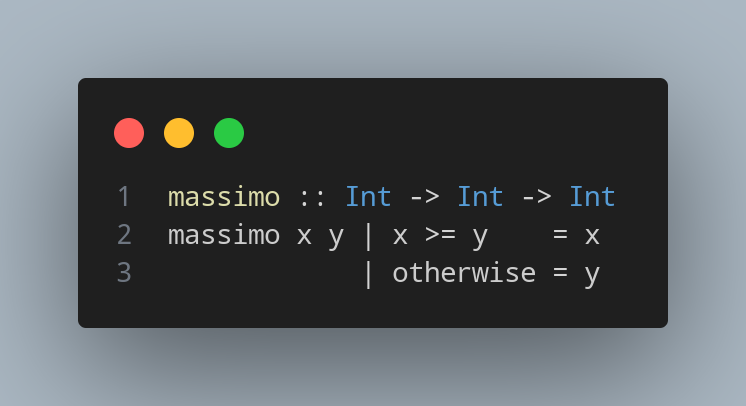
\includegraphics[width=0.5\textwidth]{images/Massimo.png}
\end{figure}

\paragraph{Massimo:} Scrivere una funzione in Haskell (con tipo \texttt{Int -> Int -> Int}), usando 
le guardie, che
prenda in input due interi e restituisca il minore.

\begin{figure}[!h]
    \centering
    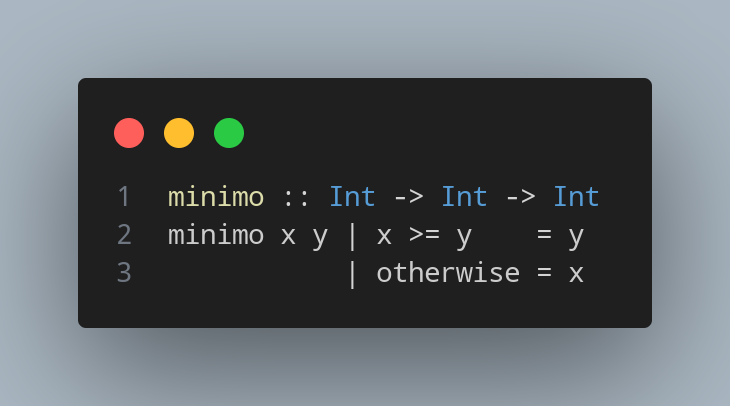
\includegraphics[width=0.5\textwidth]{images/Minimo.png}
\end{figure}

\pagebreak

\subsection{Esercizi sulle liste}

Prima di iniziare gli esercizi con le liste si deve condividere questa "dispensa"
che illustra le principali caratteristiche delle liste.

\begin{figure}[!h]
    \centering
    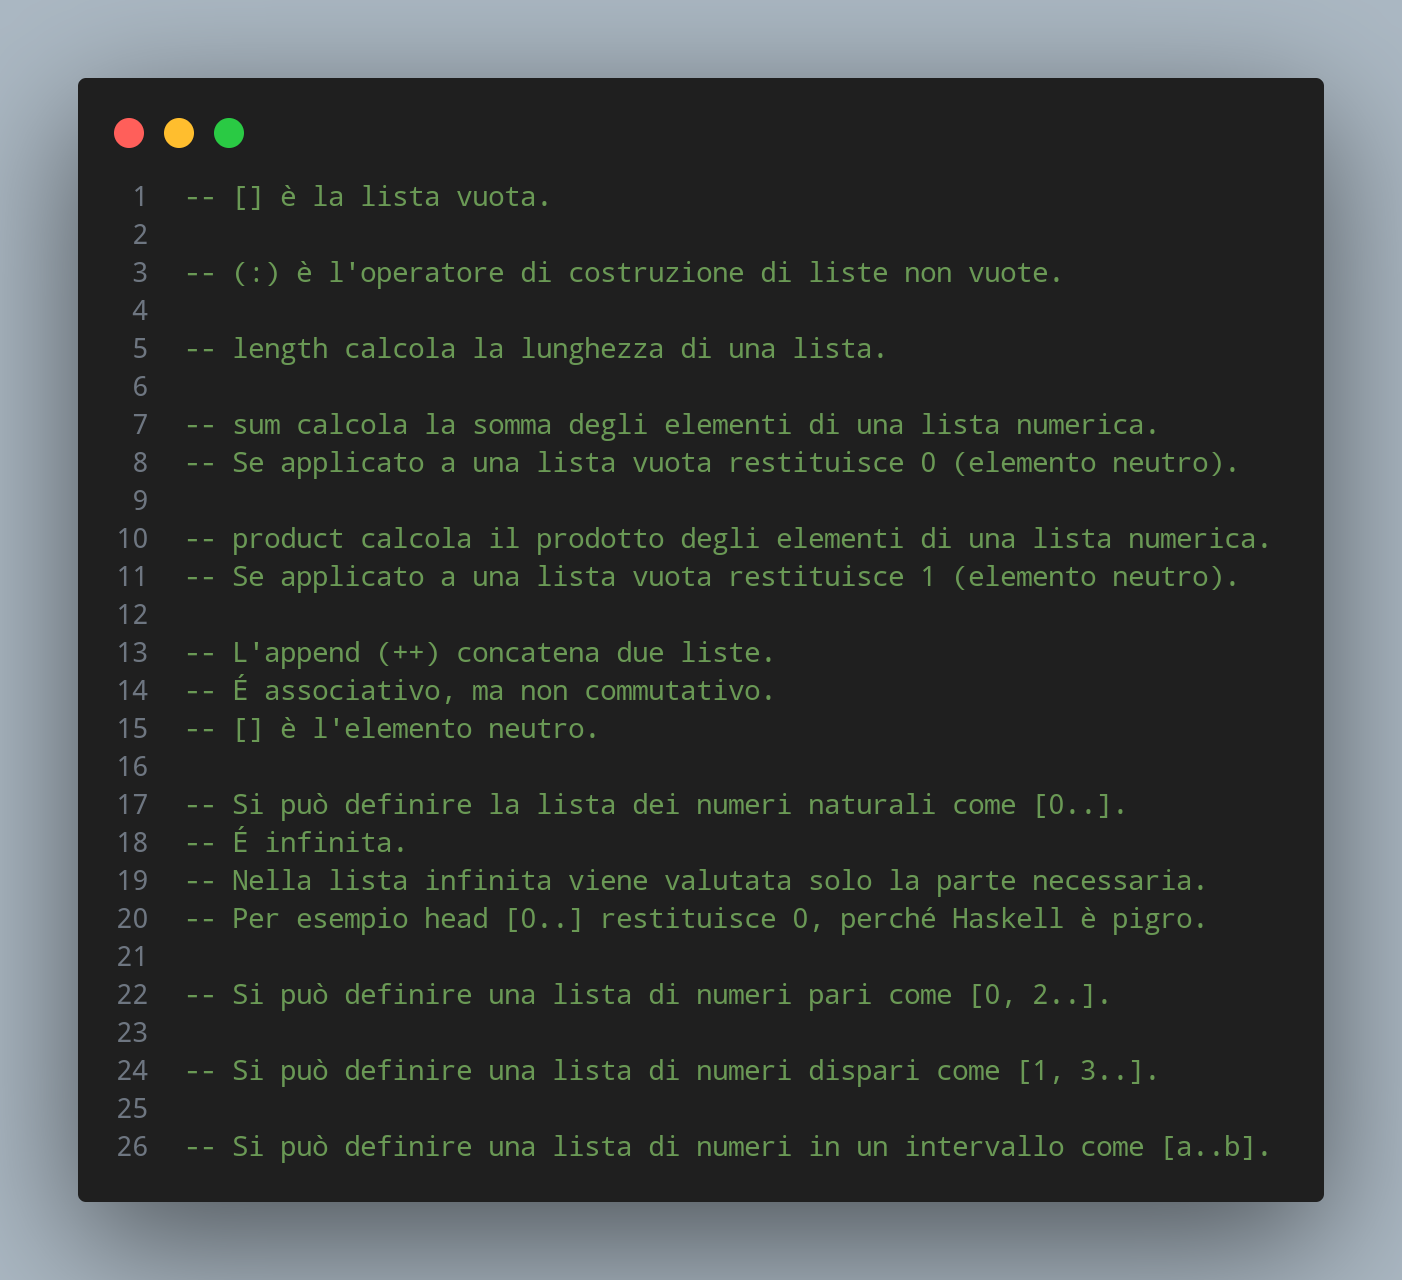
\includegraphics[width=1\textwidth]{images/Dispensa liste.png}
\end{figure}

\pagebreak

